\documentclass[10pt]{article}
\usepackage[margin=1in]{geometry}
\usepackage{amsmath, amsfonts, amsthm, amssymb}
\usepackage{tikz}
\usepackage{pseudocode}
\usetikzlibrary{trees}
\usetikzlibrary{shapes.geometric}
\usepackage[normalem]{ulem}
\usepackage{caption}
\usepackage{pgfplots}
\usepackage{listings}
\author{Hao Hou}
\title{PyTex Demo}

% these are compressed lists to help fit into a 1 page limit
\newenvironment{enumerate*}%
  {\vspace{-2ex} \begin{enumerate} %
     \setlength{\itemsep}{-1ex} \setlength{\parsep}{0pt}}%
  {\end{enumerate}}
 
\newenvironment{itemize*}%
  {\vspace{-2ex} \begin{itemize} %
     \setlength{\itemsep}{-1ex} \setlength{\parsep}{0pt}}%
  {\end{itemize}}
 
\newenvironment{description*}%
  {\vspace{-2ex} \begin{description} %
     \setlength{\itemsep}{-1ex} \setlength{\parsep}{0pt}}%
  {\end{description}}

\newenvironment{theorem}[2][Theorem]{\begin{trivlist}
\item[\hskip \labelsep {\bfseries #1}\hskip \labelsep {\bfseries #2.}]}{\end{trivlist}}
\newenvironment{lemma}[2][Lemma]{\begin{trivlist}
\item[\hskip \labelsep {\bfseries #1}\hskip \labelsep {\bfseries #2.}]}{\end{trivlist}}
\newenvironment{exercise}[2][Exercise]{\begin{trivlist}
\item[\hskip \labelsep {\bfseries #1}\hskip \labelsep {\bfseries #2.}]}{\end{trivlist}}
\newenvironment{problem}[2][Problem]{\begin{trivlist}
\item[\hskip \labelsep {\bfseries #1}\hskip \labelsep {\bfseries #2.}]}{\end{trivlist}}
\newenvironment{question}[2][Question]{\begin{trivlist}
\item[\hskip \labelsep {\bfseries #1}\hskip \labelsep {\bfseries #2.}]}{\end{trivlist}}
\newenvironment{corollary}[2][Corollary]{\begin{trivlist}
\item[\hskip \labelsep {\bfseries #1}\hskip \labelsep {\bfseries #2.}]}{\end{trivlist}}
 


\tikzset{
itria/.style={
  draw,dashed,shape border uses incircle,
  isosceles triangle,shape border rotate=90,yshift=0cm},
rtria/.style={
  draw,dashed,shape border uses incircle,
  isosceles triangle,isosceles triangle apex angle=90,
  shape border rotate=-45,yshift=0.2cm,xshift=0.5cm},
ritria/.style={
  draw,dashed,shape border uses incircle,
  isosceles triangle,isosceles triangle apex angle=110,
  shape border rotate=-55,yshift=0.1cm},
letria/.style={
  draw,dashed,shape border uses incircle,
  isosceles triangle,isosceles triangle apex angle=110,
  shape border rotate=235,yshift=0.1cm}
}

\begin{document}

\maketitle
This is a test of PyTex
Here's the Itemize

\begin{itemize}
\item \begin{tabular}{|l|l|}
\hline
$x$ & $x^2$\\
\hline
1 & 1\\
\hline
2 & 4\\
\hline
3 & 9\\
\hline
4 & 16\\
\hline
5 & 25\\
\hline
6 & 36\\
\hline
7 & 49\\
\hline
8 & 64\\
\hline
9 & 81\\
\hline
\end{tabular}
\item \begin{itemize}
\item Let's output an identity matrix
\item \begin{tabular}{ l l l l l }

1 & 0 & 0 & 0 & 0\\

0 & 1 & 0 & 0 & 0\\

0 & 0 & 1 & 0 & 0\\

0 & 0 & 0 & 1 & 0\\

0 & 0 & 0 & 0 & 1\\

\end{tabular}
\item \begin{enumerate}
\item PyTex can use this way to create a latex document
\item And we can also create new filed using program
\item For example, the next 10 line are 10 random number generated by python
\item the 0-th random number is 0.351207629222
\item the 1-th random number is 0.74917531364
\item the 2-th random number is 0.553320911684
\item the 3-th random number is 0.495962106322
\item the 4-th random number is 0.582170842076
\item the 5-th random number is 0.472835037611
\item the 6-th random number is 0.752803670144
\item the 7-th random number is 0.353354513795
\item the 8-th random number is 0.525044538949
\item the 9-th random number is 0.982742002199
\end{enumerate}
\item let's try a plot
\item 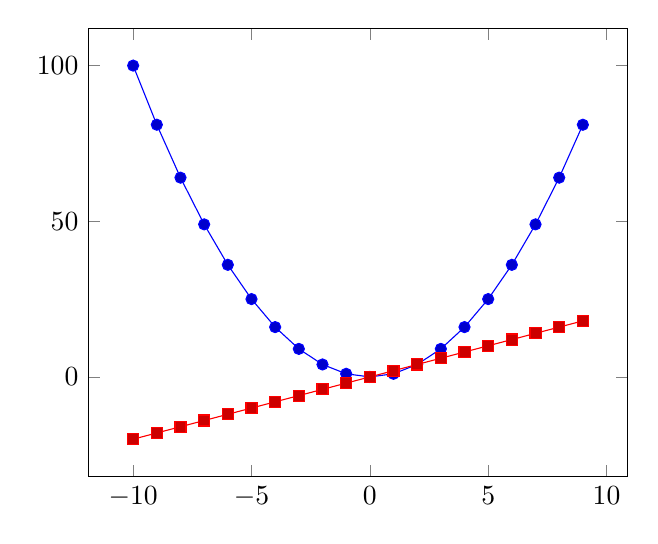
\begin{tikzpicture}
\begin{axis}
\addplot coordinates {
(-10,100)
(-9,81)
(-8,64)
(-7,49)
(-6,36)
(-5,25)
(-4,16)
(-3,9)
(-2,4)
(-1,1)
(0,0)
(1,1)
(2,4)
(3,9)
(4,16)
(5,25)
(6,36)
(7,49)
(8,64)
(9,81)
};
\addplot coordinates {
(-10,-20)
(-9,-18)
(-8,-16)
(-7,-14)
(-6,-12)
(-5,-10)
(-4,-8)
(-3,-6)
(-2,-4)
(-1,-2)
(0,0)
(1,2)
(2,4)
(3,6)
(4,8)
(5,10)
(6,12)
(7,14)
(8,16)
(9,18)
};
\end{axis}
\end{tikzpicture}
\end{itemize}
\end{itemize}

\end{document}

